% !TEX program = lualatex
\documentclass[12pt,a4paper]{article}
\usepackage{fontspec}
\setmonofont{Latin Modern Mono}
\usepackage{xcolor}
\usepackage{listings}
\usepackage{geometry}
\usepackage{fancyhdr}
\usepackage{hyperref}
\usepackage{graphicx}
\geometry{margin=1in}
\usepackage{multicol}

% -------------------------------
% SOLUTION TOGGLE
% -------------------------------
\newif\ifshowsolutions
\showsolutionstrue 
% \showsolutionsfalse

% -------------------------------
% Header and Footer Configuration
% -------------------------------
\pagestyle{fancy}
\fancyhf{}
\lhead{Lab Final}
\rhead{CSE 4308: DBMS Lab}
\cfoot{\thepage}
\setlength{\headwidth}{\textwidth}

% -------------------------------
% Code Listing Style
% -------------------------------
\definecolor{codegreen}{rgb}{0,0.6,0}
\definecolor{codegray}{rgb}{0.5,0.5,0.5}
\definecolor{codepurple}{rgb}{0.58,0,0.82}
\definecolor{backcolour}{rgb}{0.95,0.95,0.92}

\lstdefinestyle{mystyle}{
    backgroundcolor=\color{backcolour},
    commentstyle=\color{codegreen},
    keywordstyle=\color{magenta},
    numberstyle=\tiny\color{codegray},
    stringstyle=\color{codepurple},
    basicstyle=\ttfamily\footnotesize,
    breaklines=true,
    captionpos=b,
    keepspaces=true,
    numbers = none,
    numbersep=5pt,
    tabsize=2,
    frame=single,
    columns=fullflexible,
    showspaces=false,
    showstringspaces=false,
    showtabs=false
}

\lstset{style=mystyle}

% Images: found next to this file (local compile_labs.sh) or via the
% lab folder when compiled from the project root (Overleaf).
\graphicspath{{lab_14_final/}}

\begin{document}

% --------------------------------------------------------------
% TITLE PAGE
% --------------------------------------------------------------
\begin{titlepage}
    \centering
    \vspace*{2\baselineskip}

    \rule{14cm}{2pt}\vspace*{-0.8\baselineskip}\vspace*{1.5pt}
    \rule{14cm}{0.5pt}\vspace{2\baselineskip}

    {\Huge\bfseries\scshape Lab Final\par}
    \vspace{3mm}
    {\Large }
    \vspace{3mm}

    \rule{14cm}{0.5pt}\vspace*{-0.7\baselineskip}\vspace{2.5pt}
    \rule{14cm}{2pt}

    \vspace{2\baselineskip}

    {\Large\bfseries CSE 4308\par}
    \vspace{1\baselineskip}
    {\large DATABASE MANAGEMENT SYSTEMS LAB\par}

    \vfill
    {\normalsize Prepared by:\\ Samnun Azfar, Jr. Lecturer, CSE\\ Samia Nawsheen, Jr. Lecturer, CSE\par}
    {\normalsize Academic Year: AY25-26\par}
\end{titlepage}

\newpage

% ==============================================================
\section{Lab Final}

\begin{enumerate}

% ==============================================================
\item List films whose replacement cost is higher than the average replacement cost. Show title and replacement cost.

\ifshowsolutions
\begin{lstlisting}[language=SQL]
SELECT 
    title,
    replacement_cost
FROM film
WHERE replacement_cost > (
    SELECT AVG(replacement_cost)
    FROM film
)
ORDER BY replacement_cost DESC;
\end{lstlisting}
\fi

\item List films that were never rented.
Show film id and title.

\ifshowsolutions
\begin{lstlisting}[language=SQL]
SELECT f.film_id, f.title
FROM film f
LEFT JOIN inventory i ON i.film_id = f.film_id
LEFT JOIN rental r ON r.inventory_id = i.inventory_id
WHERE r.rental_id IS NULL
ORDER BY f.film_id;
\end{lstlisting}
\fi


\item List customers who have rentals from store 1 and store 2.
Show customer id and full name.

\ifshowsolutions
\begin{lstlisting}[language=SQL]
SELECT c.customer_id, c.first_name, c.last_name
FROM customer c
WHERE c.customer_id IN (
    SELECT r.customer_id
    FROM rental r
    JOIN inventory i ON i.inventory_id = r.inventory_id
    WHERE i.store_id = 1
)
AND c.customer_id IN (
    SELECT r.customer_id
    FROM rental r
    JOIN inventory i ON i.inventory_id = r.inventory_id
    WHERE i.store_id = 2
)
ORDER BY c.customer_id;
\end{lstlisting}
\fi


% ==============================================================
\item Lists all films that are currently rented, ordered the result by film\_id.

\ifshowsolutions
\begin{lstlisting}[language=SQL]
SELECT f.film_id,
       f.title,
       r.rental_id
FROM rental r
JOIN inventory i ON i.inventory_id = r.inventory_id
JOIN film f ON f.film_id = i.film_id
WHERE r.return_date IS NULL
ORDER BY f.film_id, r.rental_id;
\end{lstlisting}
\fi


\item Find films that were rented by customers from the highest 
number of different countries. Show film title and country count.

\ifshowsolutions
\begin{lstlisting}[language=SQL]
SELECT f.title,
       COUNT(DISTINCT co.country_id) AS country_count
FROM film f
JOIN inventory i ON i.film_id = f.film_id
JOIN rental r ON r.inventory_id = i.inventory_id
JOIN customer c ON c.customer_id = r.customer_id
JOIN address a ON a.address_id = c.address_id
JOIN city ci ON ci.city_id = a.city_id
JOIN country co ON co.country_id = ci.country_id
GROUP BY f.film_id, f.title
ORDER BY country_count DESC
LIMIT 5;
\end{lstlisting}
\fi


\item Write an anonymous block that prints revenue per month. Print month and total revenue using a loop.

\ifshowsolutions
\begin{lstlisting}[language=SQL]
DO $$
DECLARE
    rec RECORD;
BEGIN
    FOR rec IN
        SELECT TO_CHAR(p.payment_date, 'YYYY-MM') AS month,
               SUM(p.amount) AS revenue
        FROM payment p
        GROUP BY TO_CHAR(p.payment_date, 'YYYY-MM')
        ORDER BY month
    LOOP
        RAISE NOTICE 'Month % -> Revenue %', rec.month, rec.revenue;
    END LOOP;
END $$;
\end{lstlisting}
\fi


\item Write an anonymous block that prints the top 3 staff members by total payment collected.
Print staff id, full name, and total revenue using a loop.

\ifshowsolutions
\begin{lstlisting}[language=SQL]
DO $$
DECLARE
    rec RECORD;
    i INT := 0;
BEGIN
    FOR rec IN
        SELECT s.staff_id, s.first_name, s.last_name,
               SUM(p.amount) AS total_revenue
        FROM staff s
        JOIN payment p ON p.staff_id = s.staff_id
        GROUP BY s.staff_id, s.first_name, s.last_name
        ORDER BY total_revenue DESC, s.staff_id
    LOOP
        i := i + 1;
        EXIT WHEN i > 3;

        RAISE NOTICE '%) Staff %: % % (Revenue=%)',
            i, rec.staff_id, rec.first_name, rec.last_name, rec.total_revenue;
    END LOOP;
END $$;
\end{lstlisting}
\fi

% ==============================================================
\item Write a function that takes a film id and prints whether the film is more popular than average. Print the film title, its rental count, and the average rental count. (A film is considered more popular than average if its rental count is
greater than the average rental count per film).

\ifshowsolutions
\begin{lstlisting}[language=SQL]
DO $$
DECLARE
    v_film_id INT := 1;
    v_title TEXT;
    v_count INT;
    v_avg NUMERIC;
BEGIN
    SELECT title
    INTO v_title
    FROM film
    WHERE film_id = v_film_id;

    IF NOT FOUND THEN
        RAISE NOTICE 'Film id % not found', v_film_id;
        RETURN;
    END IF;

    SELECT COUNT(r.rental_id)
    INTO v_count
    FROM inventory i
    JOIN rental r ON r.inventory_id = i.inventory_id
    WHERE i.film_id = v_film_id;

    SELECT AVG(cnt)
    INTO v_avg
    FROM (
        SELECT COUNT(r2.rental_id) AS cnt
        FROM inventory i2
        JOIN rental r2 ON r2.inventory_id = i2.inventory_id
        GROUP BY i2.film_id
    ) sub;

    IF v_count > v_avg THEN
        RAISE NOTICE 'Film: % (id=%) Rentals=% Avg=% -> ABOVE average',
            v_title, v_film_id, v_count, ROUND(v_avg, 2);
    ELSE
        RAISE NOTICE 'Film: % (id=%) Rentals=% Avg=% -> NOT above average',
            v_title, v_film_id, v_count, ROUND(v_avg, 2);
    END IF;
END $$;
\end{lstlisting}
\fi



% ==============================================================
\item Create a function \texttt{film\_revenue\_range} that returns the total revenue earned by a given film within a given date range.
\ifshowsolutions
\begin{lstlisting}[language=SQL]
CREATE OR REPLACE FUNCTION film_revenue_range(
    p_film_id INT,
    p_from DATE,
    p_to DATE
)
RETURNS NUMERIC
LANGUAGE plpgsql
AS $$
DECLARE
    v_total NUMERIC;
BEGIN
    SELECT COALESCE(SUM(p.amount), 0)
    INTO v_total
    FROM inventory i
    JOIN rental r ON r.inventory_id = i.inventory_id
    JOIN payment p ON p.rental_id = r.rental_id
    WHERE i.film_id = p_film_id
      AND p.payment_date::date BETWEEN p_from AND p_to;

    RETURN v_total;
END;
$$;
-- Invocation (example)
SELECT film_revenue_range(1, '2007-02-14', '2007-05-14');
\end{lstlisting}
\fi


\item Create a procedure \texttt{print\_late\_days} that takes a rental id and prints how many days late it is. If the value is negative, print 0.

\ifshowsolutions
\begin{lstlisting}[language=SQL]
CREATE OR REPLACE PROCEDURE print_late_days(p_rental_id INT)
LANGUAGE plpgsql
AS $$
DECLARE
    v_rental_date DATE;
    v_duration INT;
    v_late_days INT;
BEGIN
    SELECT r.rental_date::date, f.rental_duration
    INTO v_rental_date, v_duration
    FROM rental r
    JOIN inventory i ON i.inventory_id = r.inventory_id
    JOIN film f ON f.film_id = i.film_id
    WHERE r.rental_id = p_rental_id;

    IF NOT FOUND THEN
        RAISE NOTICE 'Rental % not found', p_rental_id;
        RETURN;
    END IF;

    v_late_days := (CURRENT_DATE - v_rental_date) - v_duration;
    IF v_late_days < 0 THEN
        v_late_days := 0;
    END IF;

    RAISE NOTICE 'Rental % late days = %', p_rental_id, v_late_days;
END;
$$;

-- Example:
CALL print_late_days(1);
\end{lstlisting}
\fi

\end{enumerate}
\newpage
\section{ER Diagram}
\begin{figure}[h]
        \centering
        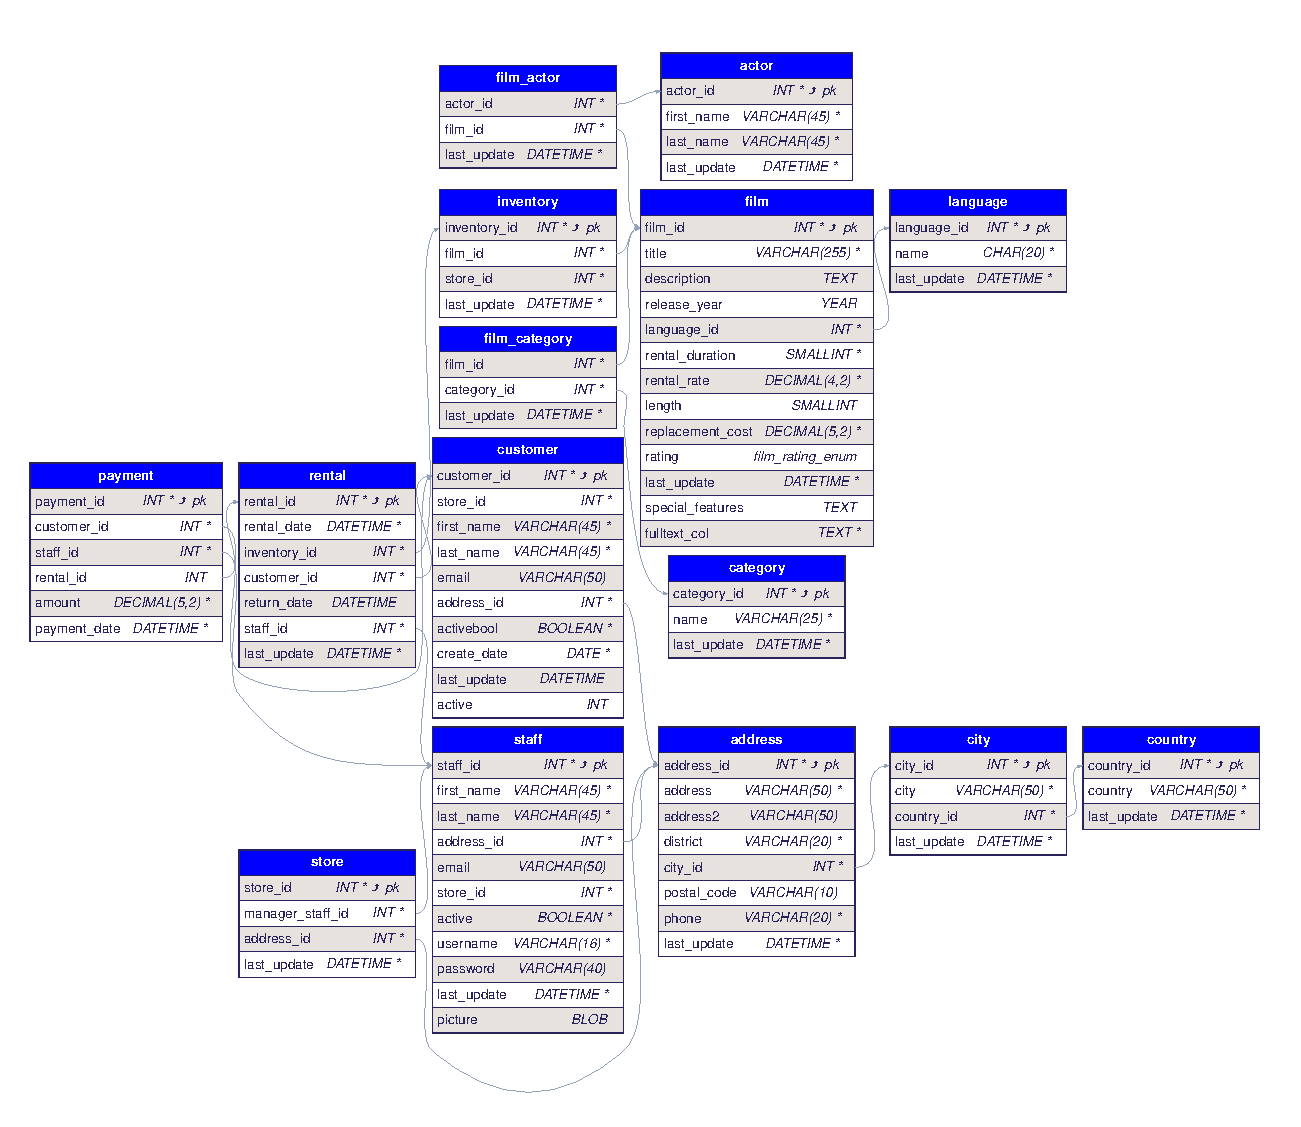
\includegraphics[width=\textheight, height=\textwidth, keepaspectratio, angle=90]{lab_14_schema_cropped.pdf}
\end{figure}

\end{document}